\documentclass[12pt, a4paper]{article}

\usepackage{graphicx}
\usepackage{amsmath}
\usepackage{algorithm}
\usepackage{algpseudocode}
\usepackage[margin=3cm]{geometry}
\usepackage{algcompatible}



\begin{document}

\tableofcontents
\newpage

\section{Problem 1 : Introduction}
\subsection{Description}

F5 : $ab^x$ is an exponential function, where a is a constant value, $a \ne 0$ and it also represents starting (initial) value , b is called base and is a positive real number and $b \ne 1$, x is called the exponent (power), it is independent variable . In this function, b is a constant value, whereas x is variable.

\subsection{Domain}

The domain for exponential function is the set of real numbers. 
\newline $x \in R$ ,  -$\infty < x <\infty$ , Domain : $\{x \mid x \in R$\}

\subsection{Co-Domain}

Co-Domain is the set of all possible function output values.
\newline Suppose $y = f(x) = ab^x $, then -$\infty < y <\infty$ , so the range will be $[-\infty,\infty]$.

\subsection{Characteristics}
\begin{itemize}
    \item In exponential function, if $ b > 0 $, then it is known as exponential growth function (increasing function). Its graphical representation shown in the left part of the figure 1.
    \item In exponential function, if $ 0 < b < 1$, then it is known as exponential decay function (decreasing function). Its graphical representation shown in the right part of the figure 1.
    \item Exponential function have horizontal asymptote (i.e function approaches to a imaginary horizontal line but never crosses) at $ Y=0 $ (i.e $ X $ – axis).
    \item They are continuous function.
    \item There is no symmetry in exponential function, so they are neither odd nor even function.
    \item Exponential function is not injective but is surjective. 
\end{itemize}

\newpage

\begin{figure}[h]
  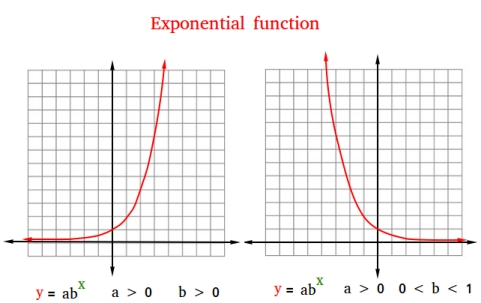
\includegraphics[width=\linewidth]{exponential-function.jpg}
  \caption{Exponential Function Graph (Growth And Decay).}
  \label{fig:exponential function graph (growth and decay)}
\end{figure}

\subsection{Context of Use Model}
\begin{figure}[h!]
  
\includegraphics[width=0.5\linewidth]{frog.jpg}
  \caption{Exponential Function Graph (Growth And Decay).}
  \label{fig:exponential function graph (growth and decay)}
\end{figure}


\newpage

\section{Problem 2 : Requirements}
\begin{enumerate}
    \item{} Requirement 1
        \begin{itemize}
        \item \textbf{ID} : R1
        \item \textbf{Version} : 1.0
        \item \textbf{Type} : Functional Requirement
        \item \textbf{Priority} : High
        \item \textbf{Difficulty} : Easy
        \item \textbf{Description} : In the exponential function $ ab^x $, the input value a should be greater than 0 i.e., $ a > 0 $ (or else it will result in output of the function to be 0 for every input), also input value of base b must be greater than 1 i.e., $ b > 1 $ (or else if $b = 1 $, it will result in output of the function to be ‘a’ for every input of x).
        \end{itemize}
    
    \item{} Requirement 2
        \begin{itemize}
        \item \textbf{ID} : R2
        \item \textbf{Version} : 1.0
        \item \textbf{Type} : Functional Requirement
        \item \textbf{Priority} : High
        \item \textbf{Difficulty} : Easy
        \item \textbf{Description} : In the exponential function $ab^x$, the input value of base b must not be negative as it will result will be complex numbers so $b > 0$.
        \end{itemize}
    
    \item{} Requirement 3
        \begin{itemize}
        \item \textbf{ID} : R3
        \item \textbf{Version} : 1.0
        \item \textbf{Type} : Functional Requirement
        \item \textbf{Priority} : High
        \item \textbf{Difficulty} : Easy
        \item \textbf{Description} : : In the exponential function $ab^x$, the input value of x must be any real number. i.e $x \in R$.
        \end{itemize}
    
    \newpage
    
    \item{} Requirement 4
        \begin{itemize}
        \item \textbf{ID} : R4
        \item \textbf{Version} : 1.0
        \item \textbf{Type} : Functional Requirement
        \item \textbf{Priority} : High
        \item \textbf{Difficulty} : Medium
        \item \textbf{Description} : The system must take input values of a, b and x from the users and return the output of $ab^x$ function. For example, if $ a = 2, b = 3 , x = 2,$ the output should be $ 18 $.
        \end{itemize}
    
    \item{} Requirement 5
        \begin{itemize}
        \item \textbf{ID} : R5
        \item \textbf{Version} : 1.0
        \item \textbf{Type} : Functional Requirement
        \item \textbf{Priority} : High
        \item \textbf{Difficulty} : Easy
        \item \textbf{Description} : If any of the input values a, b or x are not provided by the user, the system should not accept that input and ask user to provide the missing values. 
        \end{itemize}
    
    \item{} Requirement 6
        \begin{itemize}
        \item \textbf{ID} : R6
        \item \textbf{Version} : 1.0
        \item \textbf{Type} : Functional Requirement
        \item \textbf{Priority} : High
        \item \textbf{Difficulty} : Easy
        \item \textbf{Description} : If the input values are not of integer type, the system must not accept it and handle the error and ask for integer values as input.
        \end{itemize}
        
    \newpage
    
    \item{} Requirement 7
        \begin{itemize}
        \item \textbf{ID} : R7
        \item \textbf{Version} : 1.0
        \item \textbf{Type} : Functional Requirement
        \item \textbf{Priority} : Medium
        \item \textbf{Difficulty} : Easy
        \item \textbf{Description} : If the user enters any large input value which the system cannot handle, it should throw an exception and handle it accordingly.
        \end{itemize}
\end{enumerate}

\newpage

\section{Problem 3 : Algorithms}

Two algorithms (Algorithm 1 and Algorithm 2) have been selected for \newline
implementing the function $y = ab^x $. The pseudocode for each of the algorithm is provided in this section followed by their detailed description and the advantages as well as the disadvantages of each approach are discussed later.

\subsection{Algorithms and Pseudocode}
\begin{algorithm}[hbt!]
\caption{Iterative-Exponent(a,b,x)}\label{alg:one}

\hspace*{\algorithmicindent} \textbf{Input : }double number $a,b,x$ \\
\hspace*{\algorithmicindent} \textbf{Output : }value of the function $ab^x$ represented by double number result
\begin{algorithmic}[1]
\STATE $temp \gets 1$
\WHILE{$x > 0$}
  \STATE $temp \gets temp \times b$
  \STATE $x \gets x - 1$
\ENDWHILE
\STATE $result \gets a \times temp$
\STATE return $result$
\end{algorithmic}
\end{algorithm}

In this algorithm, the iterative approach is used for calculation of the given function, $ab^x$, Initially a temporary  variable called $temp$ is initialized to 1 and to calculate $b^x$, While loop is used for all the values of $x$ (exponent) and in each iteration, $temp$ is multiplied by $b$ (base) and the value of $x$ is decremented by 1. The loop continue until the exponent value $x$ reaches to 0. At last, $a$ is multiplied with the $temp$ value $(a*b^x)$ and the output is obtained in the result and it is returned.

\newpage

\begin{algorithm}[hbt!]
\caption{Recursive-Exponent(a,b,x)}\label{alg:two}

\hspace*{\algorithmicindent} \textbf{Input : }double number $a,b,x$ \\
\hspace*{\algorithmicindent} \textbf{Output : }value of the function $ab^x$ represented by double number result
\begin{algorithmic}[1]
\STATE $temp \gets recursive\_power(b,x)$
\STATE $result \gets a \times temp$
\STATE return $result$
\end{algorithmic}
\end{algorithm}



\begin{algorithm}[hbt!]
\caption{recursive\_power(b,x)}\label{alg:two}

\hspace*{\algorithmicindent} \textbf{Input : }double number $b,x$. \\
\hspace*{\algorithmicindent} \textbf{Output : }value of $b^x$ will be returned.
\begin{algorithmic}[1]
\STATE $holder \gets recursive\_power(b,x/2)$
\IF{$x$ = 0}
  \STATE return $1$
\ELSIF{$x$ = 1}
  \STATE return $b$
\ELSIF{$x$ mod 2 = 0}
  \STATE return $holder \times holder$
\ELSIF{$x > $ 0}
  \STATE return $holder \times holder \times b$
\ELSE
  \STATE return $holder \times holder {/} b$
\ENDIF
\end{algorithmic}
\end{algorithm}

In this algorithm, the recursive approach using divide and conquer strategy is used for the calculation of the given function $ab^x$. $recursive\_power(b,x)$ algorithm is used for calculating the value of $b^x$, the recursive call to the function with value base $b$ and $x = x/2$ i.e $recursive\_power(b,x/2)$ is stored in holder, so that it needs to be computed just once and can be used later on. In the base case, if the value of $x$ is 0, value $1$ is returned, otherwise, if $x=1$, value $b$ is returned, if the exponent is divisible by $2$, the algorithm recurses on $(holder * holder)$ and for odd value of exponent, it recurses on $(holder * holder * b)$, for negative value of exponent, the algorithm recurses on $(holder * holder / b)$. At last, $a$ is multiplied with the returned value from $recursive\_power(b,x)$ and the output is obtained in the $result$, and it is returned.

\newpage

\subsection{Advantages and Disadvantages}



\subsubsection{Algorithm 1}
Iterative Approach

Advantages:
\begin{enumerate}
    \item {Iterative algorithms are simple and easy to develop; they can be easily understood by the reader.}
    \item {In Iterative approach there is no overhead of function calls and they do not use stack memory and hence don’t suffer from stack overflow.}
    
\end{enumerate}

Disadvantages:
\begin{enumerate}
    \item {Some iterative algorithms are slower when compared to other approaches, Algorithm 1 which was described previously has time complexity of O(n) , so for larger inputs it is inefficient.}
    \item {If the termination condition of control variable is not defined properly, it may lead to infinite loop.}
    
\end{enumerate}

\subsubsection{Algorithm 2}
Recursive Approach 

Advantages:
\begin{enumerate}
    \item {Recursive Algorithms have less time complexity for certain problems;  Algorithm 2 which was described previously has time complexity of $O(logn)$ which is better than that of Algorithm 1.}
    \item {Recursive Algorithms are very useful in situations where particular solution is to be applied repeatedly.}
    
\end{enumerate}

Disadvantages:
\begin{enumerate}
    \item {Recursion is more difficult to understand in some algorithms and tracing them is difficult}
    \item {Recursive algorithms utilize too much memory and when the base case is not defined properly it may lead to infinite loop or crashing of the CPU.}
    
\end{enumerate}

\subsection*{Decision}
Algorithm 2 (recursive approach) would be a better option for the implementation of the function $ab^x$ as it has lower time complexity and the computation of the function must be performed quickly, so it is preferable to use the recursive algorithm rather than the iterative algorithm.


\end{document}